\chapter{Tervezés}

A tervezéshet a mellékelt UML diagramokat készítettem. A megvalósítás nagyjából követi ezt az architektúrát, pár apróbb eltéréssel és kiegészítéssel.

A projekt a printf nevet kapta.

\section{Kép betöltés, konfigurálás}

A bemeneti képeket tartalmazó és manipuláló osztályok tervezésénél különösen nagy hangsúlyt helyeztem a teljesítményre. Az \href{fig:ImageSource_uml}{ábrán} látszik, hogy a forrásfájlokat pixelenként tároljuk, és számontartjuk a hozzájuk tartozó filtereket. A filterek tudják transzformálni és manipulálni a képet (pl. méret, forgatás, maszk, segédvonalak). Az eredeti képet mindig megőrizzük, hogy a filterek ne legyenek destruktívak. Annak érdekében, hogy a filtereket ne kelljen minden egyes elérésnél újraszámolni vezettem be egy cachet. Ha változnak a filterek, a cache piszkos lesz, és a következő elérésnél újraszámolódik.

\section{Képgenerálás, algoritmusok}

A képgenerálás folyamata elsőre talán triviális. Helyezzünk el a képeinket egy rácson, aszerint elforgatva, hogy hogyan keletkezik kevesebb felesleg, figyelembe véve a margót és a térközt. A régi scriptünk is ezt az algoritmust követte, és az eredménye is megfelel az elvárásainknak. Ez mindaddig működik, amíg a forrásfájljaink méretei megegyeznek. Ha már több, különböző méretű képet kell minimális feleslegre, azaz minimális magasságú dokumentumra elhelyeznünk. Ez a probléma a ládapakolásra vezethető vissza, annak egy két dimenziós speciális esete, ahol figyelembe kell vegyük azt, hogy az eredményt vágóasztallal vágni tudjuk. Ez azt jelenti hogy a dokumentumot valahol az egyik szélétől a szemközti széléig elvágva keletkezett részek vagy egy kép, vagy egy vágóasztallal tovább vágható csík.\footnote{\href{https://en.wikipedia.org/wiki/Guillotine_cutting}{Guillotine cutting - Wikipedia}} A ládapakolás problémája viszont egy NP nehéz probléma.\footnote{\href{https://en.wikipedia.org/wiki/Bin_packing_problem}{Bin packing problem - Wikipedia}} Orbán Levente talált egy tanulmányt\footnote{\href{https://sci-hub.se/10.1016/j.ipl.2015.08.008}{A priority heuristic for the guillotine rectangular packing problem}} ennek kapcsán, ami ugyan nem mindig optimális, de az igényeinknek megfelelő polinomiális algoriutmust tartalmaz. Az algoritmusból továbbá hiányzott az is, a keletkező felesleget töltse ki oda esetleg beférő képekkel.

Ennek fényében úgy döntöttünk, hogy támogassuk mindkét megközelítést, és majd a felhasználó dönt a különböző algoritmusok között. Erre a célra szolgál egy Tiling interface, ami megkapja a képek listáját és a dokumentum tulajdonságait.

\section{A felhasználói felület}

A legnagyobb szabadságunk a felhasználói felület kapcsán volt. Mindenképpen szerettem volna egy előnézetet, hogy még mentés előtt a felhasználó lássa az eredményt, és azt esetleg javítani tudja a bemenetek újrakonfigurálásával. A kezelés lépéseinek sorrendje alapján igyekeztem kialakítani a felület többi részét. Vannak bemeneti képeink, azokat szeretnénk egyesíteni, majd kinyomtatni. Képek, egyben, nyomtatás. Ezt balról jobbra elrendezve kapjuk meg a felület végleges tervét: balra a bemenetek, azok beállításai, középen egy előnézet, jobbra pedig a kimenet (generált dokumentum) beállításai, a generálás és az exportálás/nyomtatás gomb. A UI feladata lenne továbbá az előbeállítások betöltése és a filterek beállítása is. A bemenetek alapján meghívódik a generálás, ami elkészíti nekünk a kívánt képet, ezt fogjuk látni az előnézeten.

Az említett előbeállítások valamilyen fájlból betölthető konfigurációk, melyek vonatkozhatnak a bemenő képekre, a kimenő dokumentumra, valamint esetlegesen a nyomtatóra. Ezzel megoldható, hogy ne kelljen fejben tartanunk a tekercsek és a papírok szabványainak méretét.


\begin{figure}
    \centering
    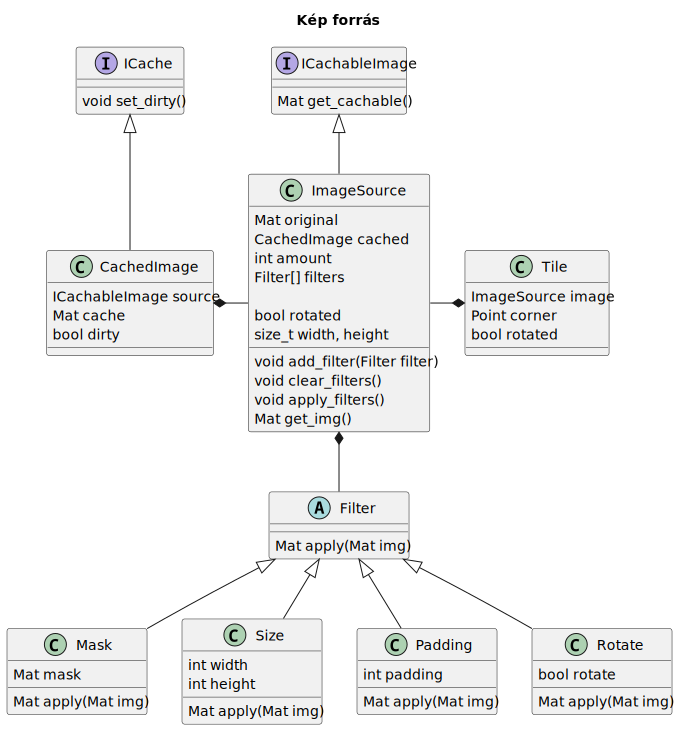
\includegraphics[width=15cm]{figures/uml/img_source.pdf}
    \label{fig:ImageSource_uml}
\end{figure}

\begin{figure}
    \centering
    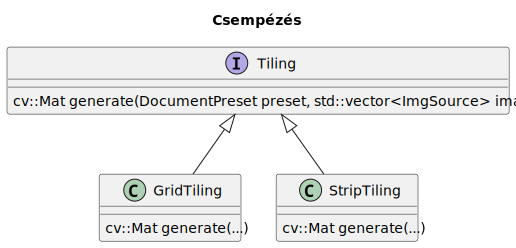
\includegraphics[width=12cm]{figures/uml/tiling.pdf}
    \label{fig:Tiling_uml}
\end{figure}

\begin{figure}
    \centering
    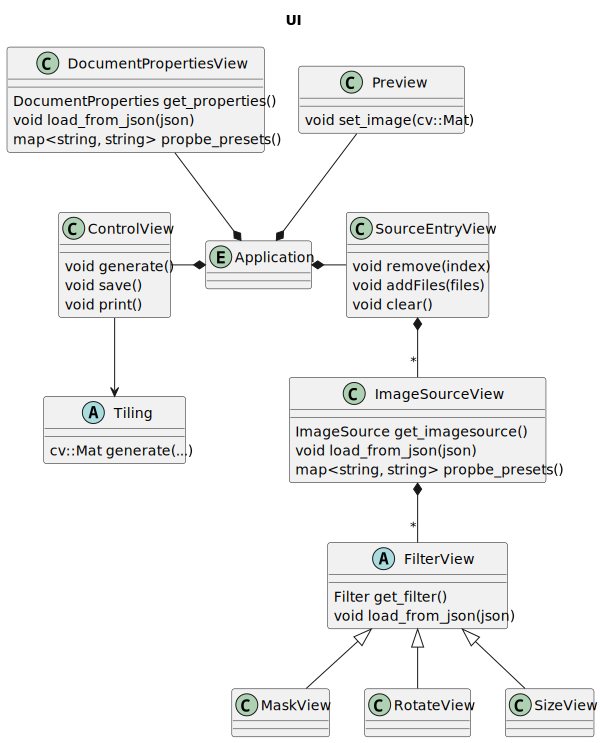
\includegraphics[width=14cm]{figures/uml/ui.pdf}
    \label{fig:UI_uml}
\end{figure}
